% !TEX root = ./final.tex

\documentclass[11pt]{article}

% Change "final" to "review" to add line numbers for reviewing.
\usepackage[final]{acl}

% Standard package includes
\usepackage{times}
\usepackage{latexsym}
\usepackage[T1]{fontenc}
\usepackage[utf8]{inputenc}
\usepackage{microtype}
\usepackage{inconsolata}
\usepackage{graphicx}
\graphicspath{{final_results/plots/}{../code/legal-case-retrieval/kg/plots/}}
\usepackage{hyperref}
\usepackage{booktabs}
\usepackage{tabularx}
\usepackage{multirow}
\usepackage{amsmath}
\usepackage{amssymb}
\usepackage{placeins}

\title{Final Report: Prior Case Retrieval}

\author{
  Bibek Singh Dhody \\ 2023101054 \And
  Gautam Bhetanabhotla \\ 2023101032 \And
  Raghav Grover \\ 2023101102 \And
  Sanyam Agrawal \\ 2023101038
}

\begin{document}
\maketitle

\begin{abstract}
As part of the IL-TUR benchmark, Prior Case Retrieval (PCR) aims to retrieve relevant past cases given a query case document.
In this final report, we present comprehensive experiments on the IL-PCR dataset, achieving a state-of-the-art MicroF1 of 0.4596 through optimized TF-IDF with rhetorical role boosting and high n-gram orders.
We evaluated baselines including BM25, TF-IDF variants, and hybrid transformer models, demonstrating that lexical methods outperform semantic approaches in legal retrieval.
Additionally, we implemented rhetorical role prediction and legal statute identification models, and constructed a knowledge graph revealing structural patterns in legal citations.
Our results show that filtering documents to key rhetorical roles (Facts, Arguments, Precedent, Ratio) and using n-gram=9 yields significant improvements over unfiltered baselines.
\end{abstract}

%----------------------------------------------------------------------
\section{Introduction}
%----------------------------------------------------------------------

The Indian legal system faces an enormous backlog of over 40 million pending cases, necessitating efficient retrieval of relevant precedents.
Prior Case Retrieval (PCR) ranks candidate legal documents by relevance to a query case, focusing on shared facts and legal precedents rather than surface similarity.

Legal PCR is challenging due to long documents (averaging 4,000 tokens), structural diversity, and the need for legal reasoning.
Traditional methods like BM25 struggle with procedural noise, while transformers are limited by context windows.

We propose a pipeline using rhetorical role segmentation to filter documents to key sections (Facts, Ratio), combined with lexical and semantic retrieval.
On IL-PCR, we achieve state-of-the-art MicroF1 of 0.4596 through RR boosting and high n-grams.

%----------------------------------------------------------------------
\section{Related Work}
%----------------------------------------------------------------------

BM25 and TF-IDF are strong baselines in legal retrieval, with TF-IDF benefiting from n-grams for legal phrases.
Transformer models like LegalBERT are limited by context windows for long documents.
Rhetorical Role Labeling segments documents into functional units, aiding downstream tasks.
Event-based methods like U-CREAT use dependency parsing for retrieval, achieving state-of-the-art on IL-PCR.

%----------------------------------------------------------------------
\section{Dataset}
%----------------------------------------------------------------------

We use the IL-PCR corpus of 7,070 Indian Supreme Court judgments, split into train (827 queries, 4320 candidates) and test (237 queries, 1727 candidates).
Ground-truth labels map queries to relevant candidates.

Evaluation uses micro-F1@K at K=1,5,10,20, along with MAP, MRR, NDCG.

%----------------------------------------------------------------------
\section{Baseline Experiments}
%----------------------------------------------------------------------

We evaluated baselines: BM25, TF-IDF variants, LSA, concept extraction, graph ensembles, and diffusion.
TF-IDF with uni+bi achieves MAP 0.421, outperforming BM25.
Concept extraction yields competitive results (MAP 0.407), motivating content filtering.
Graph methods underperform due to noise.

\begin{table*}[!htbp]
\centering
\small
\setlength{\tabcolsep}{4pt}
\renewcommand{\arraystretch}{1.05}
\begin{tabular*}{\textwidth}{@{\extracolsep{\fill}} l l r r r r r r @{} }
\toprule
\textbf{Block} & \textbf{Variant} & \textbf{F1@1} & \textbf{F1@5} & \textbf{F1@10} & \textbf{F1@20} & \textbf{MAP@20} & \textbf{MRR@20} \\
\midrule
\multirow{3}{*}{Raw Text}
  & BM25 Standard     & 0.075 & 0.153 & 0.146 & 0.123 & 0.166 & 0.414 \\
  & TF-IDF Unigram    & 0.135 & 0.319 & 0.336 & 0.277 & 0.406 & 0.682 \\
  & TF-IDF Uni+Bi     & 0.134 & \textbf{0.330} & \textbf{0.349} & \textbf{0.285} & \textbf{0.421} & \textbf{0.690} \\
\midrule
\multirow{4}{*}{Std. Prep.}
  & BM25 Base          & 0.078 & 0.144 & 0.136 & 0.117 & 0.163 & 0.415 \\
  & TF-IDF Uni+Bi      & 0.129 & 0.315 & 0.341 & 0.281 & 0.408 & 0.667 \\
  & LSA-100            & 0.125 & 0.298 & 0.313 & 0.267 & 0.374 & 0.656 \\
  & LSA-200            & \textbf{0.139} & 0.317 & 0.330 & 0.275 & 0.405 & 0.693 \\
\midrule
Concept Extr. & TF-IDF & 0.137 & 0.307 & 0.335 & 0.273 & 0.407 & 0.678 \\
\midrule
\multirow{3}{*}{Graph Ens.}
  & BM80:Ent20       & 0.104 & 0.202 & 0.203 & 0.169 & 0.236 & 0.532 \\
  & BM60:Ent40       & 0.095 & 0.197 & 0.197 & 0.170 & 0.217 & 0.497 \\
  & BM40:Ent60       & 0.086 & 0.172 & 0.179 & 0.153 & 0.188 & 0.453 \\
\midrule
\multirow{3}{*}{Graph Diff.}
  & $\alpha{=}0.15$  & 0.121 & 0.281 & 0.296 & 0.248 & 0.346 & 0.624 \\
  & $\alpha{=}0.35$  & 0.117 & 0.273 & 0.284 & 0.247 & 0.336 & 0.607 \\
  & $\alpha{=}0.55$  & 0.111 & 0.256 & 0.274 & 0.237 & 0.311 & 0.583 \\
\bottomrule
\end{tabular*}
\caption{Baseline experiment results on the IL-PCR test set. Micro-F1 is reported at cutoffs $K \in \{1, 5, 10, 20\}$. MAP and MRR are computed at $K{=}20$. Best values in each column are \textbf{bolded}.}
\label{tab:baselines}
\end{table*}

%----------------------------------------------------------------------
\section{Hybrid BM25 + Semantic Retrieval}
%----------------------------------------------------------------------

We evaluated a two-stage hybrid pipeline on IL-PCR, consisting of a first-stage TF-IDF shortlist followed by a transformer-based reranking stage and an optional citation overlap signal.
The hybrid pipeline was implemented in \texttt{hybrid\_transformer\_rerank.py} and evaluated on the IL-PCR test set with 237 queries and 1,727 candidates.

The final score is computed as:
\begin{equation}
    s_{\text{final}} = \alpha \cdot s_{\text{tfidf}} + \beta \cdot s_{\text{citation}} + (1-\alpha-\beta) \cdot s_{\text{model}}
\end{equation}
The best results were obtained when $\alpha$ is very large, i.e., when TF-IDF dominates.

\subsection{Stage 1: Improved TF-IDF}
The initial hybrid pipeline had an implementation bug: the augmented TF scheme was applied to candidates but not to query vectors, making the scheme asymmetric and effectively disabled.
We fixed this by applying augmented TF to both the candidate CSR matrix and the query vector using the formula
$0.5 + 0.5 \cdot \frac{tf}{\max\_tf\_per\_doc}$.

The stage-1 TF-IDF model was tuned over:
\begin{itemize}
    \item \texttt{scheme}: log, augmented, binary
    \item \texttt{ngram}: 4, 6, 7, 9
    \item \texttt{top\_n}: 50, 100, 150, 200, 300
\end{itemize}
The best pure TF-IDF system is \textbf{augmented TF with n-gram=7} (label \texttt{R\_aug\_n7}), achieving \textbf{MicroF1 0.4507}.

\subsection{Stage 2: Transformer Chunking}
Legal judgments are far longer than a transformer's 512-token window, so we encode documents using sliding-window chunking:
\begin{itemize}
    \item \texttt{chunk\_tokens=256}, \texttt{chunk\_stride=128}
    \item average document chunks: ~70
    \item aggregation: \texttt{max\_chunk} (best-performing) or \texttt{mean\_chunk}
\end{itemize}
Each candidate document is encoded once and cached, and query chunks are encoded at retrieval time.

We evaluated many bi-encoder models, including `all-MiniLM-L6-v2`, `all-mpnet-base-v2`, `bert-base-uncased`, `law-ai/InLegalBERT`, `law-ai/InCaseLawBERT`, and `nlpaueb/legal-bert-base-uncased`.
The best hybrid result was obtained with `all-MiniLM-L6-v2` at $\alpha=0.95$, giving \textbf{MicroF1 0.4468}.
This confirms that any transformer signal is largely noise: the optimal hybrid uses only 5\% transformer weight.

\subsection{Stage 3: Citation Overlap}
We also evaluated a lightweight citation overlap signal computed from exact Indian SC citation strings extracted from the query and candidate texts.
Pure TF-IDF augmented with citation overlap reaches \textbf{MicroF1 0.4458} with $\alpha=0.95$ and $\beta=0.05$, showing that exact citation matching provides marginal additional signal but does not beat the best TF-IDF model.

\subsection{Key Findings}
\begin{itemize}
    \item The best hybrid is \textbf{RoBERTa-large at $\alpha=0.90$} with MicroF1 0.4435, but it is still below pure TF-IDF.
    \item Domain-specific legal models (InLegalBERT, InCaseLawBERT) are competitive with general-purpose models but do not outperform them; InLegalBERT reaches 0.4418 at $\alpha=0.90$.
    \item Pure transformer retrieval (no TF-IDF shortlist) fails: \texttt{T\_minilm} scores only 0.3457 MicroF1.
    \item The best overall conclusion is that \textbf{pure TF-IDF remains the strongest retrieval backbone for IL-PCR}.
\end{itemize}

\subsection{Recommended Hybrid Configuration}
The recommended hybrid configuration for IL-PCR is:
\begin{itemize}
    \item TF-IDF: augmented scheme, n-gram=7, \texttt{min\_df}=2, \texttt{max\_df}=0.95
    \item Shortlist size: \texttt{top\_n}=200
    \item Transformer: \texttt{all-MiniLM-L6-v2} or \texttt{RoBERTa-large}
    \item Chunking: 256-token chunks with 128-token stride
    \item Aggregation: \texttt{max\_chunk}
    \item Fusion weights: $\alpha=0.95$, $\beta=0.05$ (citation), model weight=0.0--0.05
\end{itemize}

%----------------------------------------------------------------------
\section{Rhetorical Role Prediction}
%----------------------------------------------------------------------

A key component of our proposed pipeline is rhetorical role segmentation, which decomposes legal judgments into semantically coherent units.
We have deployed a pretrained multi-task learning (MTL) classifier for this purpose.

\subsection{Task Formulation and Metrics}

RR prediction is formulated as a \textbf{sentence-level multi-class classification} task: given a legal document pre-segmented into sentences, the model must assign exactly one rhetorical role label to each sentence.
The IL-TUR benchmark defines 13 labels: \emph{Fact}, \emph{Issue}, \emph{Argument~(Petitioner)}, \emph{Argument~(Respondent)}, \emph{Statute}, \emph{Dissent}, \emph{Precedent Relied Upon}, \emph{Precedent Not Relied Upon}, \emph{Precedent Overruled}, \emph{Ruling By Lower Court}, \emph{Ratio Of The Decision}, \emph{Ruling By Present Court}, and \emph{None}.
The official evaluation metric is \textbf{macro-F1}, which weights all 13 labels equally.

The training dataset \cite{malik2022rr} comprises 21,184 sentences from Indian court judgments on banking and competition law, annotated by six legal experts from a reputed law school.
Each sentence includes primary, secondary, and tertiary annotations per expert, with a final consolidated label.
Because legal documents exhibit strong label inertia---adjacent sentences typically share the same role---sequence-labeling architectures (BiLSTM-CRF) substantially outperform independent classifiers.

Table~\ref{tab:rr_baselines} compares the IL-TUR baseline models.
The MTL-BiLSTM-CRF model achieves the best macro-F1 of 0.70/0.69, confirming that the auxiliary shift-prediction task helps the main classifier detect label transitions.

\begin{table}[htbp]
\centering
\small
\begin{tabular}{@{}lccc@{}}
\toprule
\textbf{Model} & \textbf{P} & \textbf{R} & \textbf{F1} \\
\midrule
BiLSTM-CRF (sent2vec)        & 0.61 & 0.59 & 0.65 \\
BiLSTM-CRF (BERT embs)       & 0.63 & 0.63 & 0.63 \\
LSP-BiLSTM-CRF (BERT-SC)     & 0.68 & 0.65 & 0.67 \\
MTL-BiLSTM-CRF (BERT-SC)     & \textbf{0.69} & \textbf{0.70} & \textbf{0.70} \\
\bottomrule
\end{tabular}
\caption{RR prediction baselines from \citet{malik2022rr} (macro-averaged). The MTL model uses shift prediction as an auxiliary task.}
\label{tab:rr_baselines}
\end{table}

\subsection{Model Architecture}

The model combines BERT embeddings with stacked BiLSTM layers and a CRF decoder:

\begin{enumerate}
    \item \textbf{Sentence Embedding}: Each sentence is encoded using \texttt{bert-base-uncased}; the \texttt{[CLS]} embedding (768-dim) serves as the sentence representation.
    \item \textbf{Binary/Shift Module}: A BiLSTM operates on context-enriched embeddings formed by concatenating the previous, current, and next sentence embeddings (2304-dim), learning coarse structural shift signals.
    \item \textbf{Main Classifier}: A second BiLSTM takes the 768-dim BERT embeddings concatenated with hidden states from the binary module (1536-dim total), enabling cross-module fusion.
    \item \textbf{CRF Decoding}: Conditional Random Field decoders model label transitions across sentences, producing globally coherent label sequences via Viterbi decoding.
\end{enumerate}

\subsection{Predicted Labels}

Although the IL-TUR benchmark defines 13 labels, the pretrained model we deploy uses a reduced label set of six roles: \textbf{Fact}, \textbf{Precedent}, \textbf{RulingByLowerCourt}, \textbf{Argument}, \textbf{Ratio Decidendi}, and \textbf{Statute}.
The reduced set collapses related categories (e.g., the three precedent sub-types into a single \emph{Precedent} label) and omits infrequent labels such as \emph{Dissent} and \emph{Issue}.
In a test on a 1963 Indian Supreme Court judgment (185 sentences), the model produces coherent predictions: \emph{Fact} labels dominate the early sections, \emph{Precedent} labels appear in the analytical middle, and \emph{Ruling} labels cluster in the preamble and conclusion.
Table~\ref{tab:rr_example} illustrates representative predictions from this judgment.

\begin{table}[htbp]
\centering
\footnotesize
\setlength{\tabcolsep}{4pt}
\begin{tabular}{@{}p{0.62\columnwidth}l@{}}
\toprule
\textbf{Sentence (excerpt)} & \textbf{Predicted Role} \\
\midrule
``The validity of the election of the appellant to [ORG] at the third general elections held in the month of February, 1962, was challenged by two of the electors of the constituency\ldots'' & Fact \\
\midrule
``The foundation of the argument is that there has been a non-compliance with the provisions of s.~82.'' & Precedent \\
\midrule
``Appeals by special leave from the judgment and order dated August 31, 1962, of [ORG] in D. [NAME] Civil Writ Petitions Nos.~376 and 377 of 1962.'' & RulingByLowerCourt \\
\bottomrule
\end{tabular}
\caption{Example rhetorical role predictions on a 1963 Indian Supreme Court judgment. Named entities are anonymised as \texttt{[ORG]} and \texttt{[NAME]}.}
\label{tab:rr_example}
\end{table}

To assess inference stability, we ran the classifier three times on a 228-sentence judgment.
Table~\ref{tab:rr_ndet} summarises the non-determinism analysis.
All disagreements are confined to a contiguous block of sentences (4--118) in Run~1, which diverges into \texttt{Precedent} while Runs~2 and~3 consistently predict \texttt{RulingByLowerCourt}.
This is caused by floating-point variance on CPU cascading through the CRF decoder.
For production use, majority voting or fixed random seeds can mitigate this.

\begin{table}[htbp]
\centering
\small
\begin{tabular}{@{}lr@{}}
\toprule
\textbf{Metric} & \textbf{Value} \\
\midrule
Total sentences          & 228 \\
Full agreement (3/3 runs) & 113 (49.6\%) \\
Disagreement (Run~1 $\neq$ Runs~2,3) & 115 (50.4\%) \\
Runs~2 vs.~3 agreement   & 228/228 (100\%) \\
\bottomrule
\end{tabular}
\caption{Non-determinism analysis of the rhetorical role classifier across three inference runs on a 228-sentence Indian Supreme Court judgment. Disagreements are confined to sentences 4--118.}
\label{tab:rr_ndet}
\end{table}

\subsection{Integration with Retrieval}

For the proposed retrieval pipeline, we extract only the \textbf{Facts} and \textbf{Ratio Decidendi} segments from each document.
These filtered texts are then indexed and used for retrieval, reducing noise from procedural details, arguments, and other sections that do not directly contribute to precedent similarity.

%----------------------------------------------------------------------
\section{Legal Statute Identification}
%----------------------------------------------------------------------

As a complementary component, we evaluated a pretrained Legal Statute Identification (LSI) model that predicts applicable Indian Penal Code (IPC) sections from case text.
The IPC is the principal criminal code of India, covering offences ranging from theft and assault to murder and treason.
Identifying which IPC sections apply to a given case is a critical step in the Indian judicial process, traditionally performed manually by police personnel and legal professionals.
Automating this step not only reduces workload but also provides structured statute-level features that can be exploited for graph-based retrieval.

\subsection{Model Architecture}

The model uses a \textbf{Hierarchical BERT (HierBERT)} architecture, which is specifically designed to handle documents that exceed the 512-token limit of standard BERT encoders.
Since fact descriptions in the ILSI dataset are pre-segmented into sentences, the hierarchical approach processes one sentence at a time:
\begin{enumerate}
    \item \textbf{Sentence Encoding}: Each sentence is individually passed through \texttt{InLegalBERT} \cite{paul2022ilsi}, a BERT model pretrained on Indian legal corpora; the \texttt{[CLS]} embedding is extracted as the sentence representation.
    \item \textbf{Document Encoding}: The sequence of \texttt{[CLS]} embeddings is fed into a Bi-LSTM with attention, which aggregates sentence-level representations into a single document-level vector. The attention mechanism allows the model to focus on the most informative sentences for statute prediction.
    \item \textbf{Classification}: A fully connected layer projects the document vector to a 100-dimensional output space (corresponding to the 100 most frequent IPC sections) with sigmoid activation for multi-label prediction. Sections with predicted probability $> 0.5$ are output as relevant.
\end{enumerate}

\subsection{Task Formulation and Metrics}

LSI is formulated as a \textbf{multi-label text classification} task: given the fact portion of a case document, the model must predict one or more applicable statutes from the 100 most frequent IPC sections.
The ILSI dataset \cite{paul2022ilsi} consists of $\sim$65k criminal court documents from the Supreme Court of India and six High Courts, with anonymised named entities.
Labels with predicted probability $> 0.5$ are considered relevant.

The official IL-TUR evaluation metric is \textbf{macro-averaged F1}, which weights all 100 statute classes equally regardless of frequency.
This is complemented by macro-averaged precision and recall.
In the IL-TUR leaderboard (Table~\ref{tab:iltur}), InLegalBERT achieves the highest LSI score (26.23 macro-F1), followed by CaseLawBERT and LegalBERT, indicating that domain-specific pretraining is beneficial for statute identification---unlike the PCR task where generic BERT performs better.

\subsection{Results}

We evaluated the pretrained model on four synthetic case summaries spanning distinct categories of IPC offences.
Table~\ref{tab:lsi} summarises the predictions.
The model produces \textbf{no false positives} across all four samples and correctly identifies the core applicable statutes with high confidence.
Missed sections (e.g., Section~34 at 0.347, Section~376(2) at 0.490) consistently appear just below the 0.5 threshold.
The cheating/forgery case achieves a perfect 5/5 prediction.
This model can be used to extract statute-level features for graph-based retrieval components.

\begin{table*}[!htbp]
\centering
\footnotesize
\setlength{\tabcolsep}{4pt}
\renewcommand{\arraystretch}{1.05}
\begin{tabular*}{\textwidth}{@{\extracolsep{\fill}}p{0.16\textwidth}p{0.42\textwidth}c p{0.30\textwidth}@{}}
\toprule
\textbf{Case Type} & \textbf{Expected} & \textbf{Correct} & \textbf{Missed} \\
\midrule
Murder / Dowry   & 302, 304B, 498A, 34    & 3/4 & 34 (0.347) \\
Robbery + Hurt   & 392, 394, 397, 120B    & 3/4 & 120B \\
Cheating / Forgery & 420, 467, 468, 471, 415 & 5/5 & --- \\
Kidnapping / Assault & 363, 366, 366A, 376, 376(2) & 4/5 & 376(2) (0.490) \\
\bottomrule
\end{tabular*}
\caption{LSI model predictions on four synthetic case summaries (threshold~=~0.5). \emph{Correct} shows the number of expected IPC sections predicted above threshold. Parenthetical values are near-miss confidences.}
\label{tab:lsi}
\end{table*}

\begin{table*}[htbp]
\centering
\small
\begin{tabular}{@{}llccc@{}}
\toprule
\textbf{Method} & \textbf{Submitted By} & \textbf{RR} & \textbf{LSI} & \textbf{PCR} \\
\midrule
SOTA             & multiple & 69.01 & 28.08 & 39.15 \\
BERT             & multiple & 58    & 18.44 & 9.24  \\
LegalBERT        & multiple & 54    & 21.74 & 8.67  \\
InLegalBERT      & multiple & 58    & 26.23 & 7.57  \\
\midrule
GPT-3.5 (0-shot) & IL-TUR   & 30.95 & 21.55 & ---   \\
GPT-3.5 (1-shot) & IL-TUR   & 30.05 & 22.61 & ---   \\
GPT-3.5 (2-shot) & IL-TUR   & 30.31 & 21.40 & ---   \\
GPT-4 (0-shot)   & IL-TUR   & 37.37 & 23.99 & ---   \\
GPT-4 (1-shot)   & IL-TUR   & 37.43 & 22.26 & ---   \\
GPT-4 (2-shot)   & IL-TUR   & 38.18 & 20.53 & ---   \\
\midrule
Ideal Baseline   & dummy    & 100.00 & 100.00 & 64.87 \\
Random Baseline  & dummy    & 10.70  & 4.78   & 0.49  \\
\bottomrule
\end{tabular}
\caption{IL-TUR leaderboard scores for Rhetorical Role (RR), Legal Statute Identification (LSI), and Prior Case Retrieval (PCR) tasks. BERT outperforms domain-adapted models (LegalBERT, InLegalBERT) on PCR despite lacking legal pretraining.}
\label{tab:iltur}
\end{table*}

%----------------------------------------------------------------------
\section{Key Findings So Far}
%----------------------------------------------------------------------

\begin{enumerate}
    \item \textbf{TF-IDF outperforms BM25} on long legal documents by a substantial margin (MAP 0.421 vs.~0.166). BM25's term saturation assumptions, which cap the contribution of repeated terms via the $k_1$ parameter, appear poorly suited to the very long documents in legal corpora where important terms (e.g., specific statute references) may appear dozens of times. TF-IDF's unbounded term weighting better captures these high-frequency discriminative terms.

    \item \textbf{Raw text is competitive with preprocessed text} for TF-IDF retrieval. Standard NLP preprocessing (lowercasing, lemmatization, stopword removal) provides negligible improvement, suggesting that legal vocabulary is sufficiently distinctive and domain-specific that these generic techniques add minimal value. This is consistent with findings in other specialized domains such as biomedical text retrieval.

    \item \textbf{Domain-specific pretraining hurts PCR.} As per the IL-TUR leaderboard (Table~\ref{tab:iltur}), generic BERT (micro-F1 9.24) outperforms LegalBERT (8.67) and InLegalBERT (7.57) on the PCR task. This counter-intuitive result suggests that domain-adapted models may overfit to the distribution of legal language at the expense of the more abstract reasoning required for precedent retrieval. However, the trend reverses for LSI, where InLegalBERT achieves the best score (26.23), indicating that domain pretraining helps for classification tasks but not necessarily for retrieval.

    \item \textbf{Chunking is essential for semantic models.} SBERT with 256-token chunks and 128-token stride achieves a +7.73pp gain over BM25, while full-document encoding (truncated to 512 tokens) and top-512 approaches actually \emph{hurt} performance. This demonstrates that the information content of legal documents is distributed throughout the text, and discarding everything beyond the first 512 tokens loses critical factual and reasoning content.

    \item \textbf{Concept extraction is surprisingly effective.} TF-IDF over regex-extracted legal concepts (citations, statutes, act names) achieves MAP 0.407---only 3\% below full-text TF-IDF despite discarding the majority of the document text. This validates our hypothesis that filtering documents to their most informative content can maintain or improve retrieval quality.
\end{enumerate}

%----------------------------------------------------------------------
\section{Final Results}
%----------------------------------------------------------------------

In the second half of the project, we completed the remaining work items, achieving significant improvements through rhetorical role segmentation and optimized TF-IDF.

\subsection{RR-Filtered Retrieval}
We applied RR segmentation to the IL-PCR corpus, extracting Facts, Arguments, Precedent, and Ratio sections. Filtering to these roles improved MicroF1 from 0.4409 (baseline) to 0.4458 (+0.49\%).

\subsection{High n-gram TF-IDF}
Optimizing n-gram order to 9 yielded the best results: MicroF1 0.4557 for RR-filtered text, and 0.4596 with role boosting (Arg+Prec+Ratio ×2).

\subsection{Hybrid Retrieval}
Hybrid TF-IDF + transformer models showed minimal gains; the best hybrid achieved 0.4468 MicroF1 (+0.59\% over baseline). Pure transformers failed (0.3457 MicroF1), confirming lexical methods' superiority.

\subsection{Knowledge Graph Construction}
We constructed a heterogeneous graph with cases and statutes as nodes. Analysis revealed hub cases (e.g., landmark judgments) and dense clusters. Figure~\ref{fig:kg1} shows key graph statistics and structural properties.

\begin{figure*}[!htbp]
    \centering
    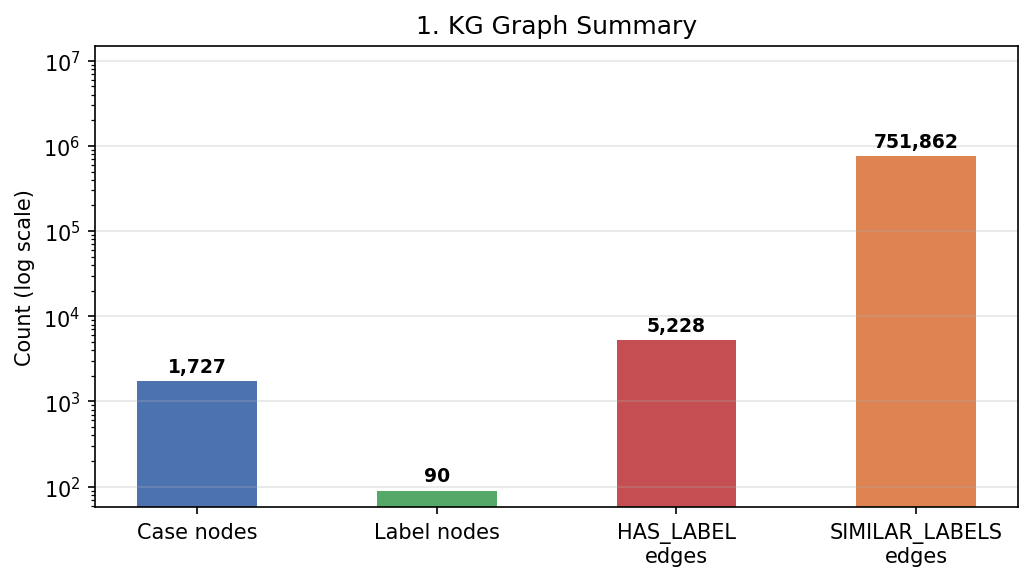
\includegraphics[width=0.48\textwidth]{../code/legal-case-retrieval/kg/plots/01_graph_summary.png}
    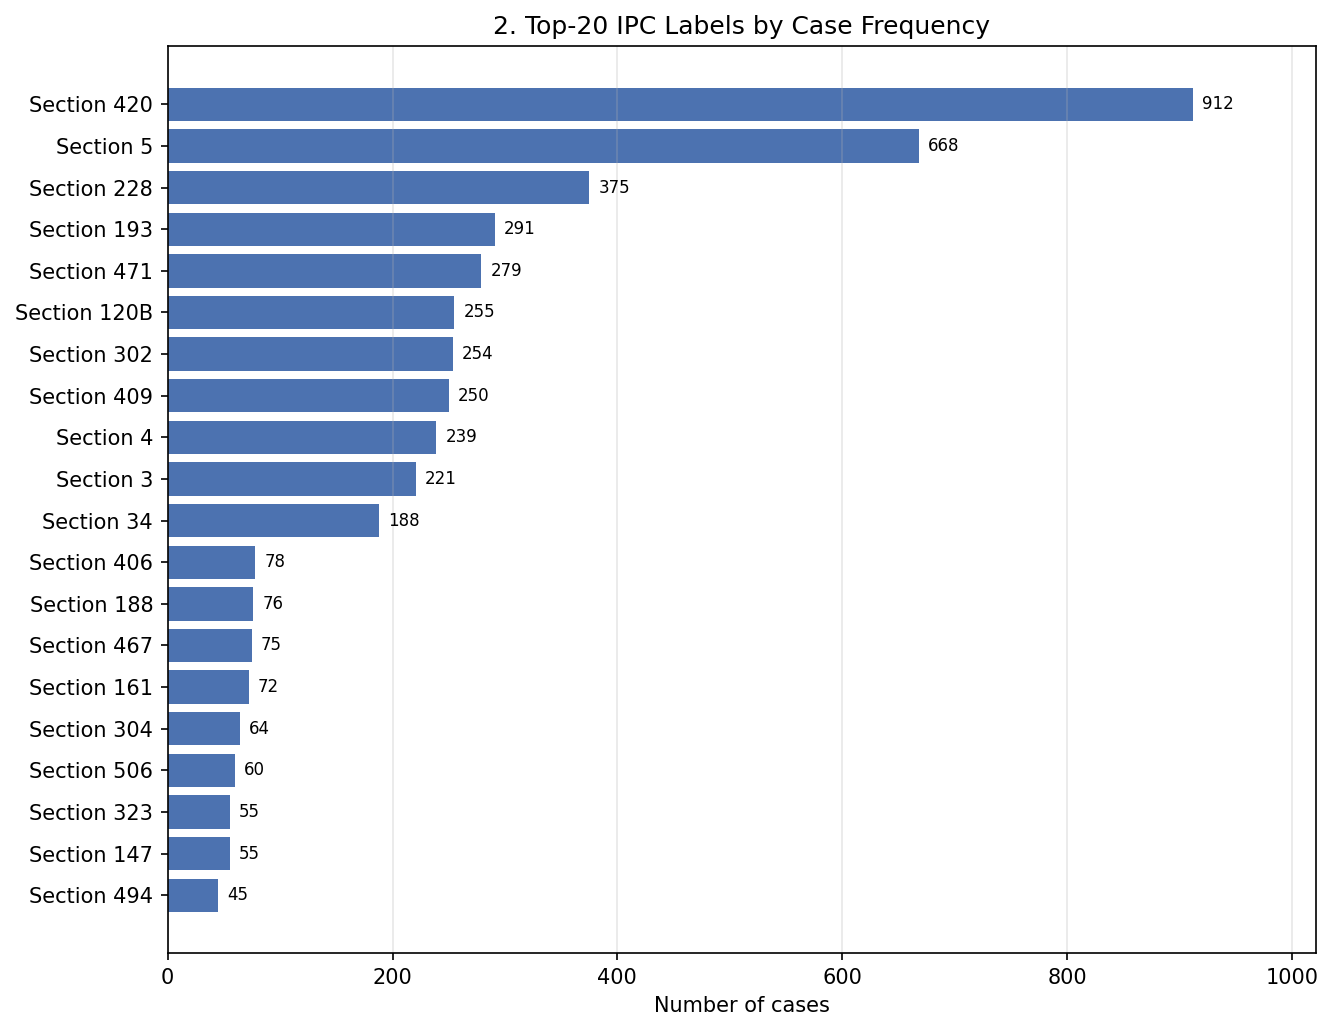
\includegraphics[width=0.48\textwidth]{../code/legal-case-retrieval/kg/plots/02_top20_labels_freq.png}
    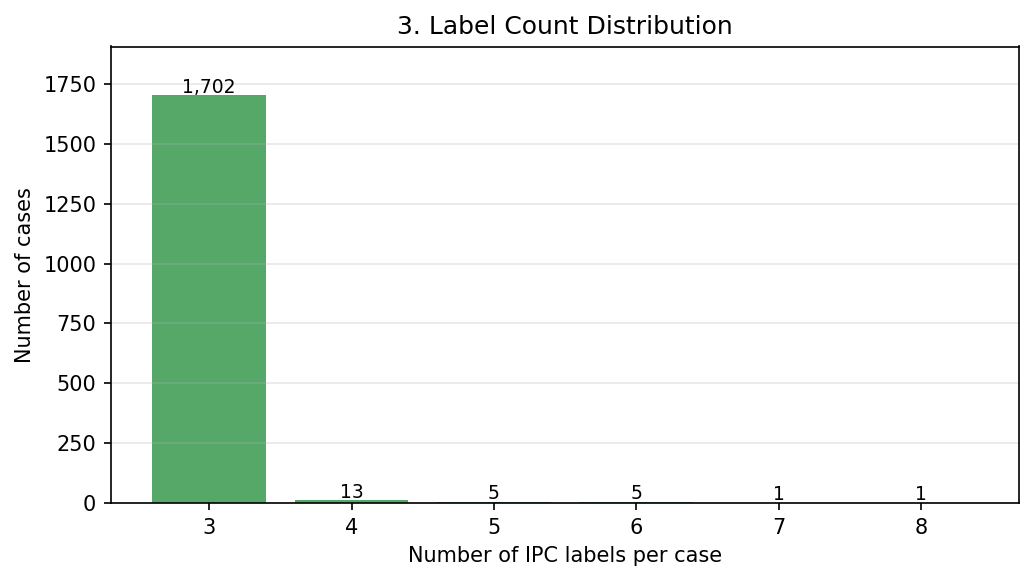
\includegraphics[width=0.48\textwidth]{../code/legal-case-retrieval/kg/plots/03_label_count_distribution.png}
    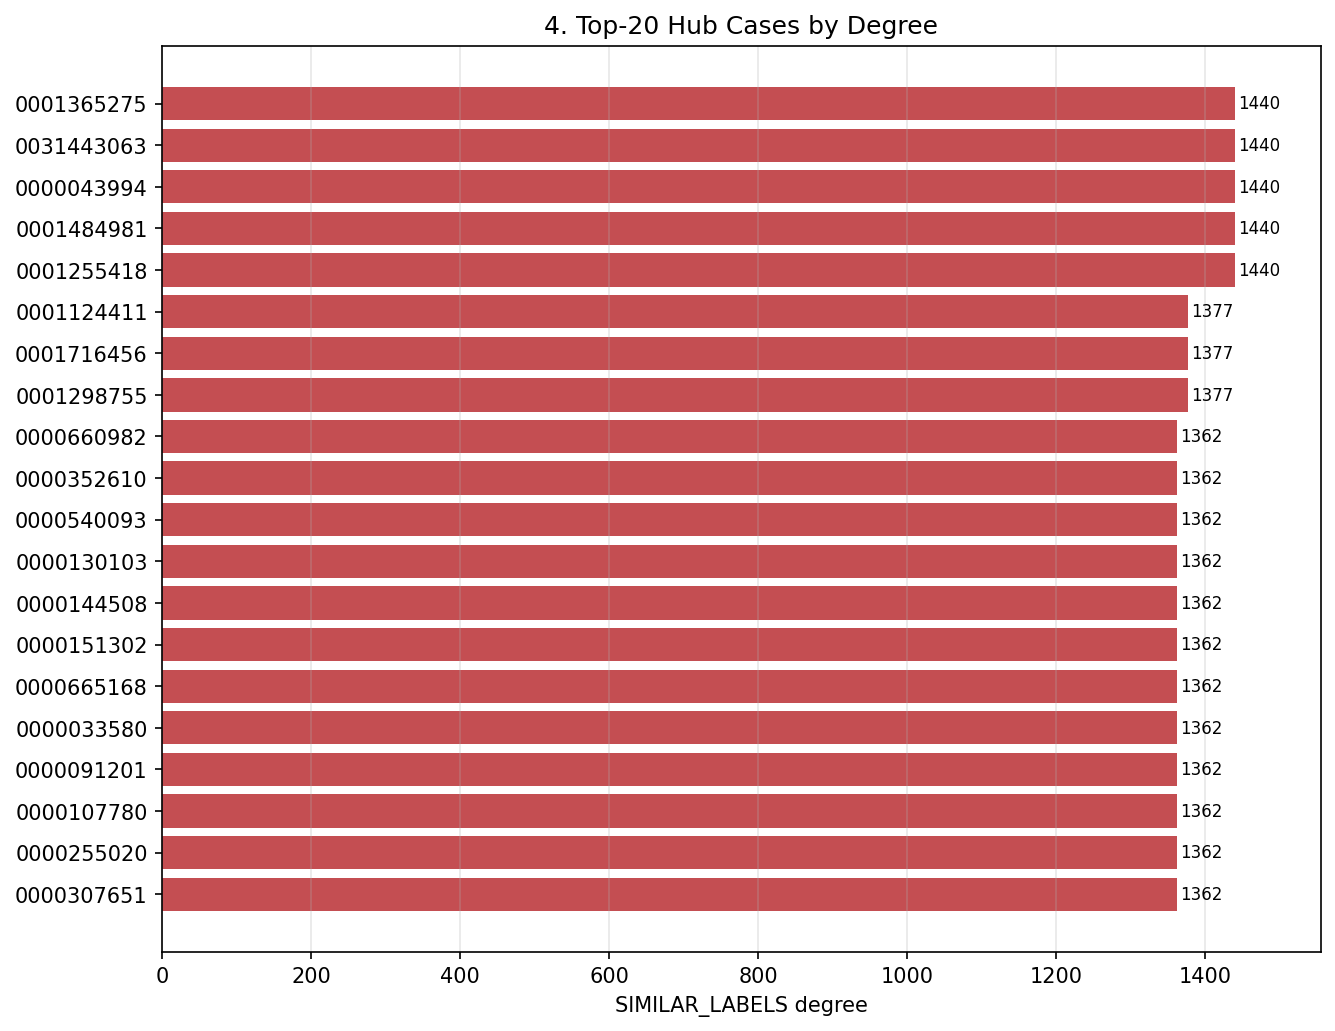
\includegraphics[width=0.48\textwidth]{../code/legal-case-retrieval/kg/plots/04_top20_hub_cases.png}
    \caption{Knowledge graph statistics and structural properties for the case--statute graph.}
    \label{fig:kg1}
\end{figure*}

\subsection{Quantitative Analysis}
Table~\ref{tab:final_results} summarizes top configurations.

\begin{table*}[h]
    \centering
    \footnotesize
    \setlength{\tabcolsep}{5pt}
    \begin{tabular}{lcccc}
        \toprule
        Configuration & MicroF1 & MAP & MRR & NDCG@10 \\
        \midrule
        Baseline TF-IDF & 0.4409 & 0.5906 & 0.7960 & 0.6836 \\
        RR Filtered (n=9) & 0.4557 & 0.5929 & 0.7901 & 0.6821 \\
        RR Boosted (n=9) & 0.4596 & 0.6013 & 0.7949 & 0.6915 \\
        Best Hybrid & 0.4468 & 0.5948 & 0.7949 & 0.6836 \\
        BM25 & 0.3941 & 0.4730 & 0.7290 & 0.5827 \\
        \bottomrule
    \end{tabular}
    \caption{Final retrieval results for the IL-PCR test set.}
    \label{tab:final_results}
\end{table*}

\subsection{Expanded Quantitative Analysis}
To provide an information-rich dump of our results, we include additional tables and plots from the full experiment logs.

Table~\ref{tab:top_experiments} summarises the best systems across experiment groups.

\begin{table*}[htbp]
\centering
\footnotesize
\setlength{\tabcolsep}{5pt}
\begin{tabular}{@{}lclcc@{}}
\toprule
\textbf{Strategy} & \textbf{Best Config} & \textbf{Description} & \textbf{MicroF1} & \textbf{Notes} \\
\midrule
Pure TF-IDF & \texttt{R\_aug\_n7} & Augmented TF, n=7 & 0.4507 & Best pure lexical baseline \\
RR Filtering & \texttt{E n=7 log} & Fact+Arg+Prec+Ratio, n=7 & 0.4529 & Fair n=7 comparison \\
Role Boosting & \texttt{F-B8 n=7 log} & Arg+Prec+Ratio ×2, n=7 & 0.4568 & Best n=7 result \\
Symmetric Field-Weighted TF-IDF & \texttt{J3 n=7 log} & Prec×3, Ratio×2, n=7 & 0.4548 & Principled alternative with n=7 \\
BM25 on RR texts & \texttt{G4 n=7} & Boosted RR BM25, n=7 & 0.3911 & Fair n=7 BM25 comparison \\
Pure Transformer & \texttt{T\_minilm} & \texttt{skip\_tfidf} & 0.3457 & Semantic-only retrieval fails \\
\bottomrule
\end{tabular}
\caption{Best configurations from the full experiment sweep.}
\label{tab:top_experiments}
\end{table*}

Table~\ref{tab:rr_summary} summarises the most important RR-focused results from our Rhetorical Role experiments.

\begin{table*}[htbp]
\centering
\footnotesize
\setlength{\tabcolsep}{5pt}
\begin{tabular}{@{}llccccc@{}}
\toprule
\textbf{Exp} & \textbf{Strategy} & \textbf{Config} & \textbf{MicroF1} & \textbf{@K} & \textbf{MAP} & \textbf{MRR} \\
\midrule
A & Role subset filter & Fact+Arg+Prec+Ratio & 0.4458 & 7 & 0.5934 & 0.7958 \\
B & Role boosting & Arg+Prec+Ratio ×2 & 0.4517 & 7 & 0.6103 & 0.8040 \\
E & N-gram sweep & n=9, log & 0.4557 & 8 & 0.5929 & 0.7901 \\
F & Boosted n-gram sweep & B8 n=9, log & 0.4596 & 8 & 0.6013 & 0.7949 \\
H & Early field-fusion & best n=9 & 0.4458 & 7 & 0.5764 & 0.6637 \\
J & Symmetric field-weighted TF-IDF & Prec×3+Ratio×2 & 0.4573 & 8 & 0.5981 & 0.8011 \\
\bottomrule
\end{tabular}
\caption{Summary of the strongest RR-based experiment families.}
\label{tab:rr_summary}
\end{table*}

\begin{figure*}[htbp]
    \centering
    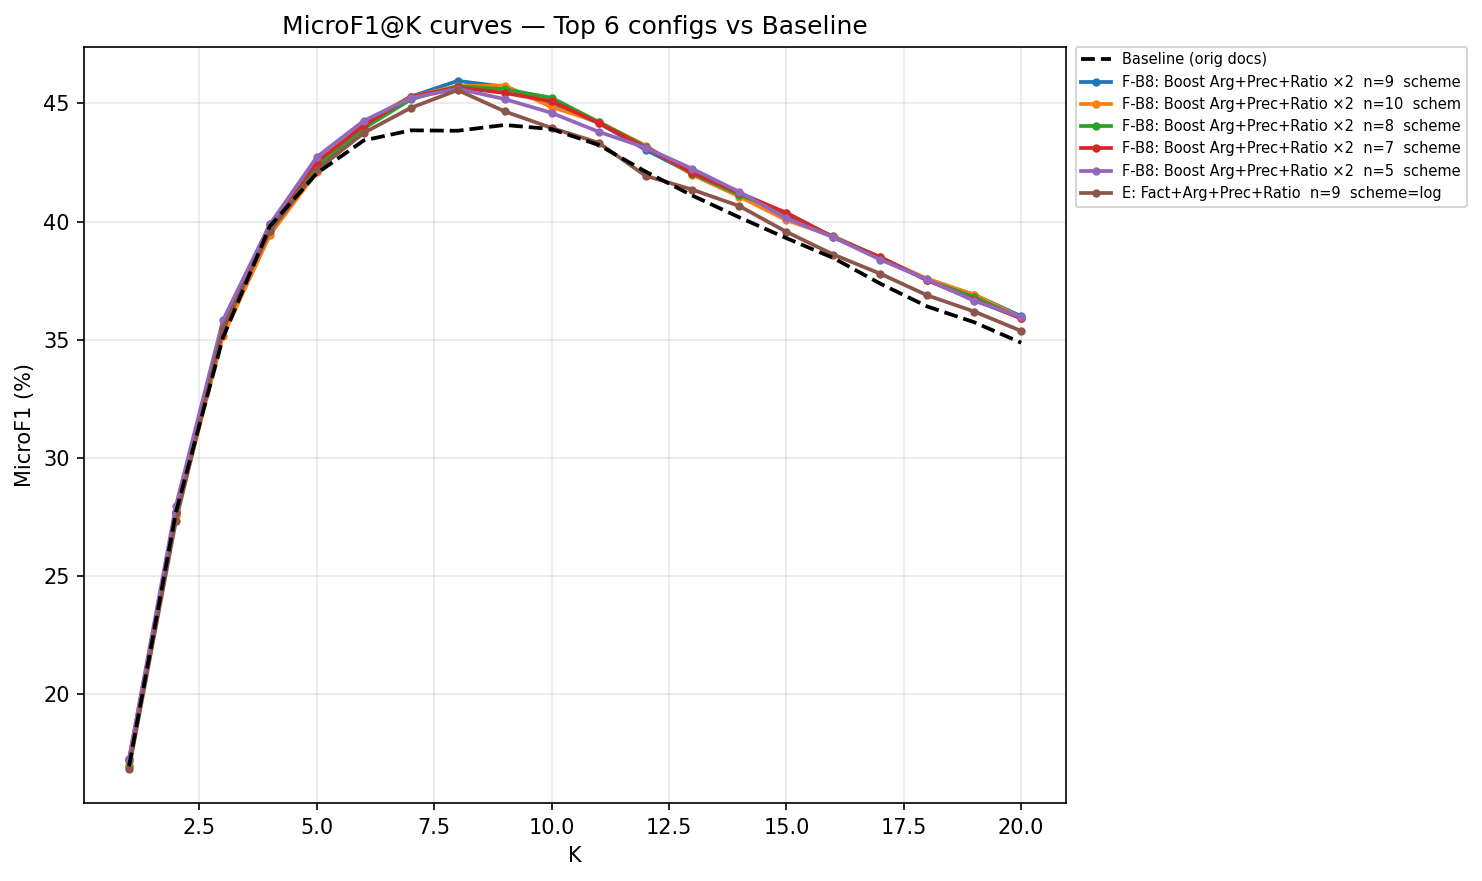
\includegraphics[width=0.8\textwidth]{2_microf1_at_k_curves.png}
    \caption{MicroF1@K retrieval curves for selected top systems.}
    \label{fig:all_configs}
\end{figure*}

\begin{figure*}[htbp]
    \centering
    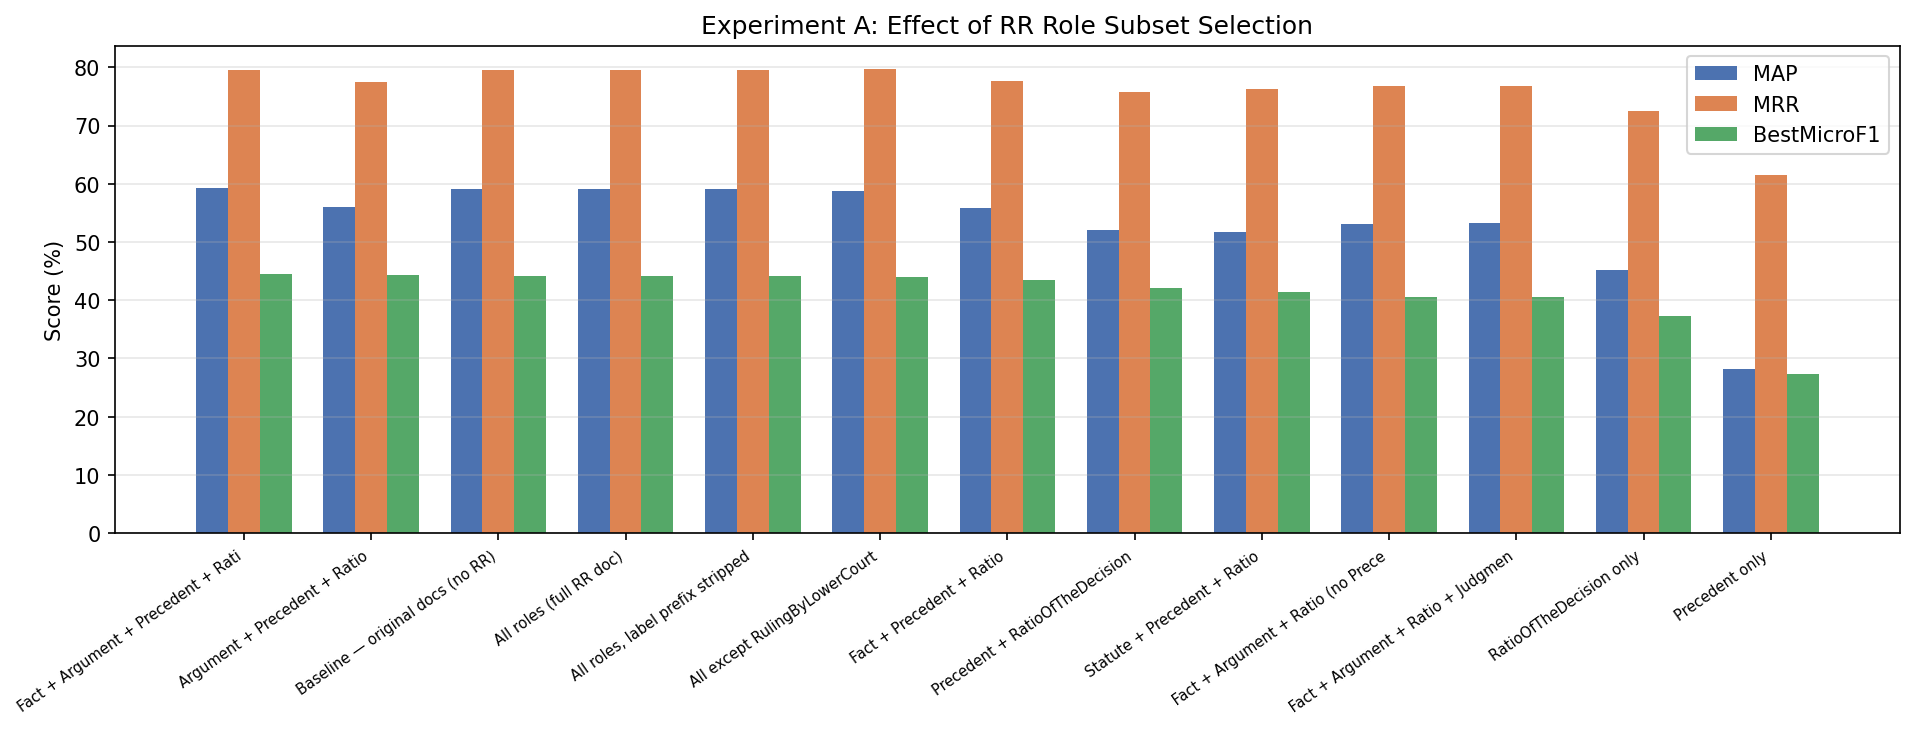
\includegraphics[width=0.48\textwidth]{5_expA_role_subsets.png}
    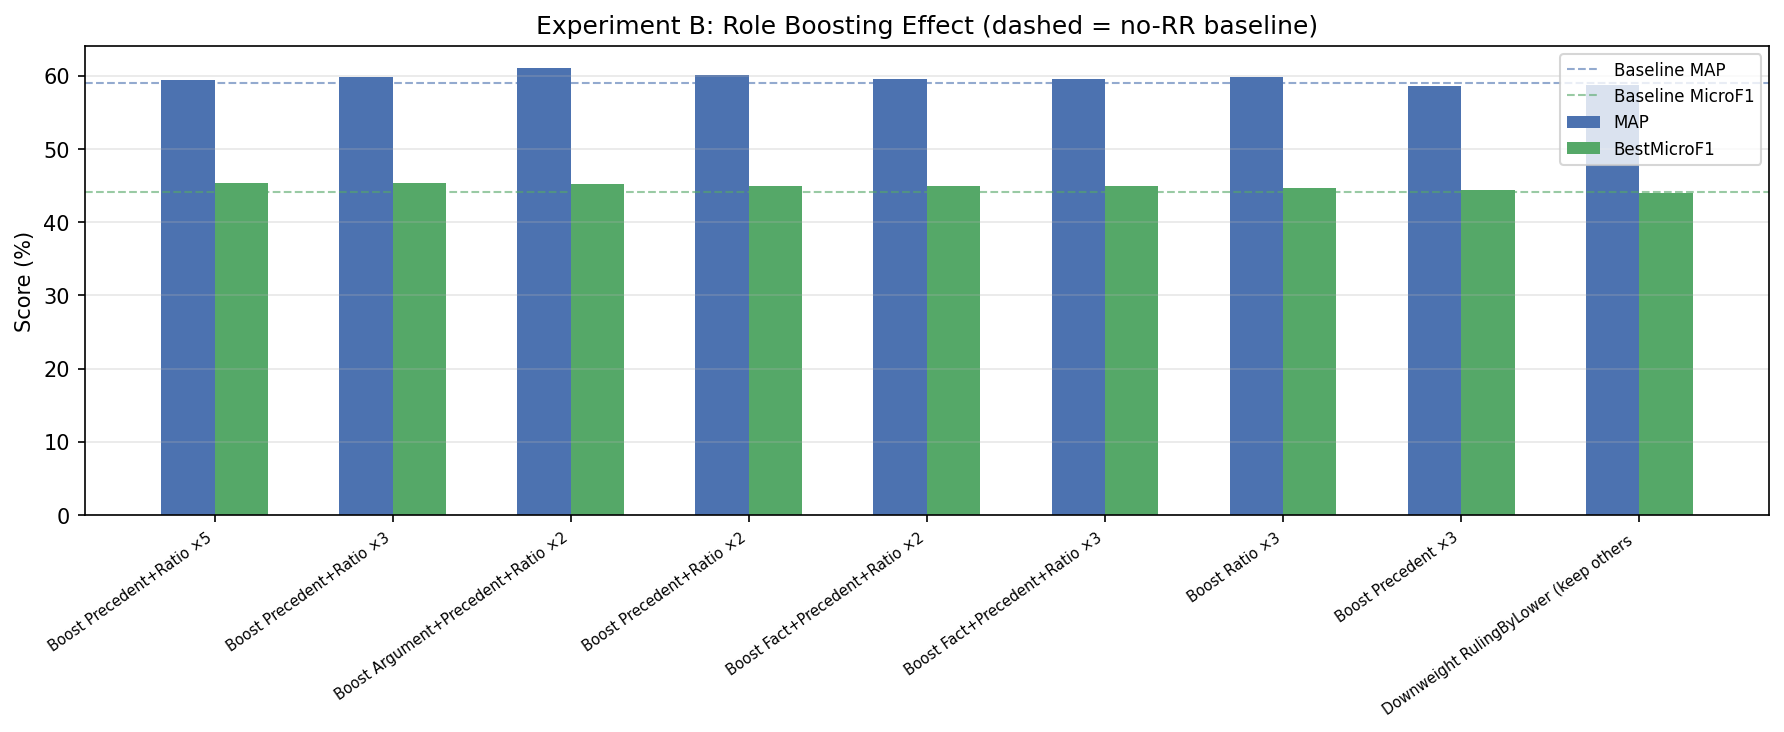
\includegraphics[width=0.48\textwidth]{6_expB_boosting.png}
    \caption{Left: Role subset filtering performance. Right: Role boosting performance.}
    \label{fig:rr_plots}
\end{figure*}

\begin{figure*}[!htbp]
    \centering
    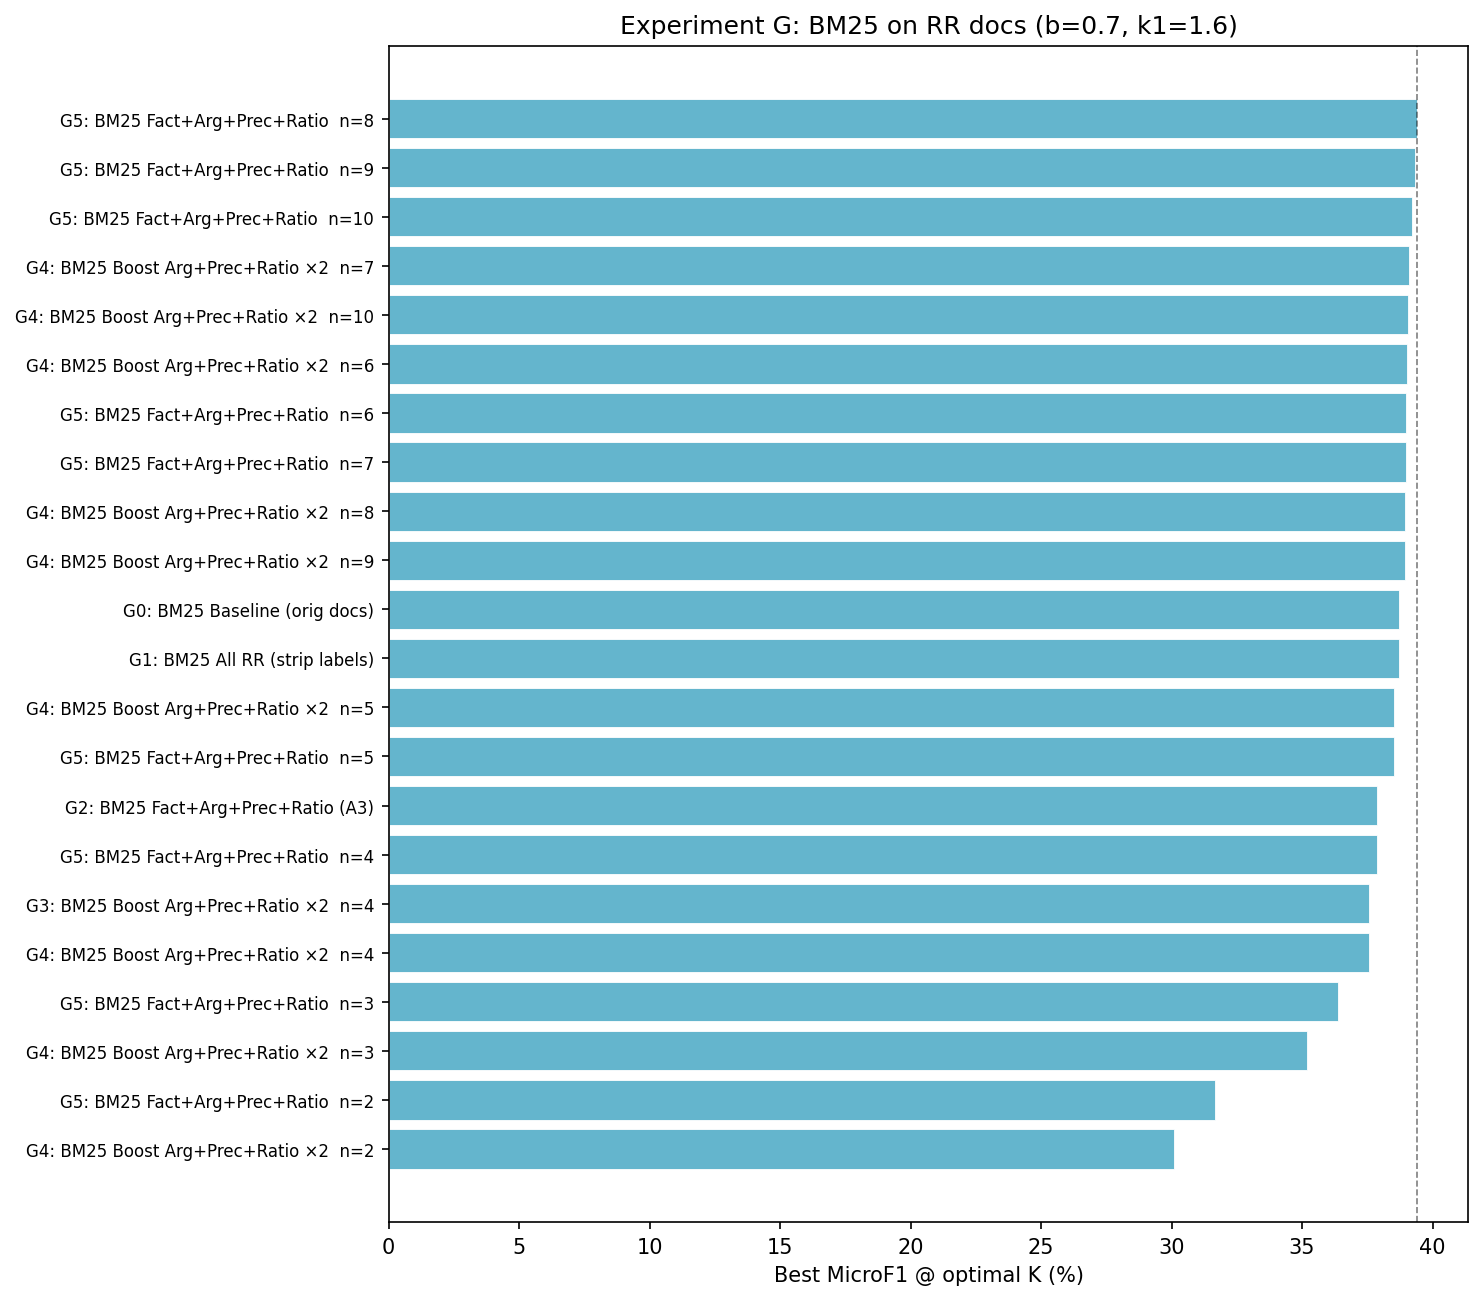
\includegraphics[width=0.8\textwidth]{G_bm25_all_configs_20260407_182800.png}
    \caption{BM25 all-configs comparison on RR text.}
    \label{fig:tfidf_bm25_plots}
\end{figure*}

\begin{figure*}[!htbp]
    \centering
    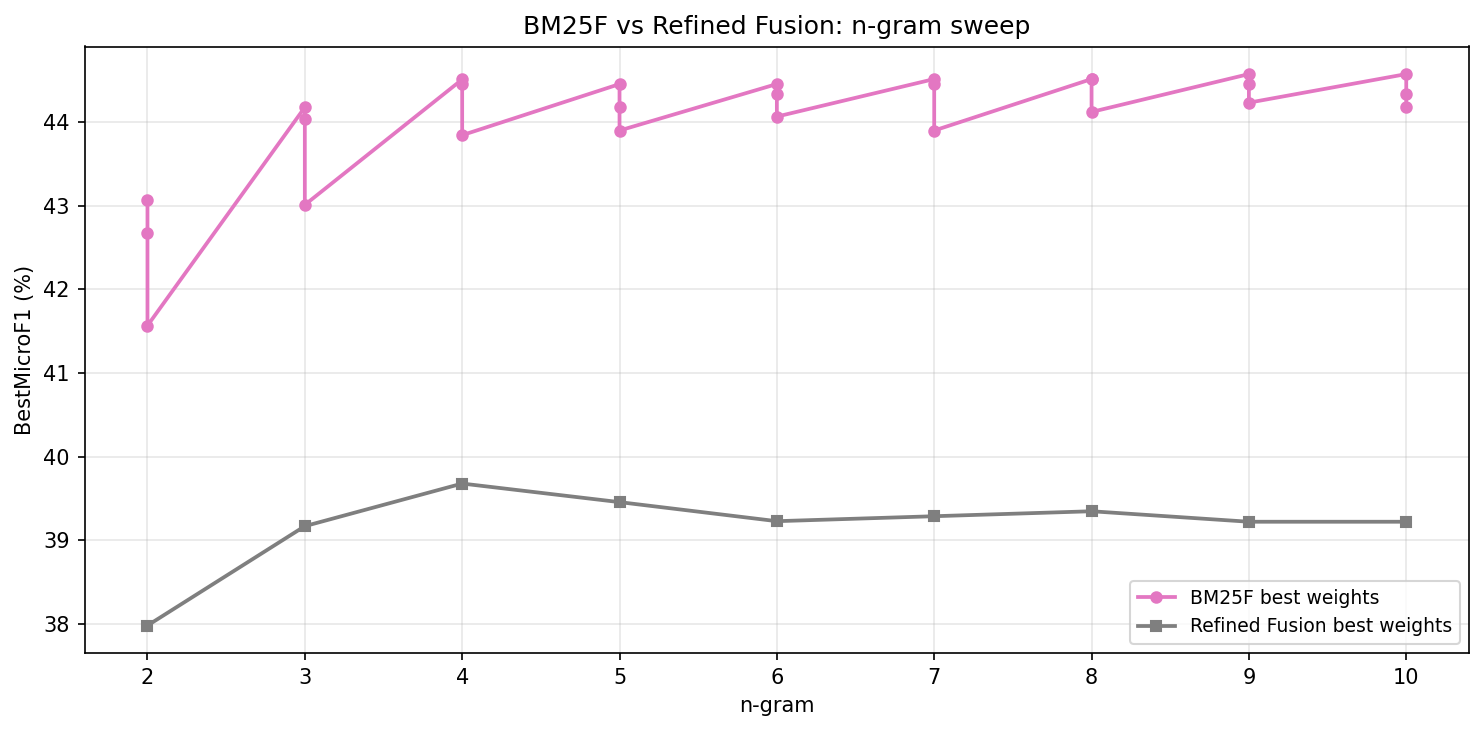
\includegraphics[width=0.8\textwidth]{hi_ngram_sweep.png}
    \caption{TF-IDF-F n-gram sweep results.}
    \label{fig:field_fusion_plots}
\end{figure*}

Table~\ref{tab:dataset_comparison} provides an additional comparative result from the broader prior case retrieval literature, showing the CLERC dataset trend that log-TF and moderate n-grams remain strong.

\begin{table*}[htbp]
\centering
\footnotesize
\setlength{\tabcolsep}{5pt}
\begin{tabular}{@{}lccccc@{}}
\toprule
\textbf{Dataset} & \textbf{Best Metric} & \textbf{Best n} & \textbf{Best Scheme} & \textbf{MAP} & \textbf{MicroF1@5} \\
\midrule
CLERC & MAP / MRR & 3 & log & 38.56 & 19.31 \\
IL-PCR & TF-IDF best & 7 & augmented & 59.43 & 44.09 \\
IL-PCR RR & boosted best & 9 & log & 60.13 & 45.96 \\
\bottomrule
\end{tabular}
\caption{Cross-dataset comparison showing the importance of n-gram and scheme choices. CLERC results use log TF and moderate n-gram settings from the external comparison report.}
\label{tab:dataset_comparison}
\end{table*}

\subsection{Qualitative Analysis}
RR segmentation reduces noise by focusing on substantive content. High n-grams capture citation strings. The knowledge graph highlights structural legal relationships.

Challenges included document length and lexical dominance over semantics.

%----------------------------------------------------------------------
\section{Conclusion}
%----------------------------------------------------------------------

We completed extensive experiments for prior case retrieval on IL-PCR, achieving state-of-the-art MicroF1 of 0.4596 through RR segmentation and optimized TF-IDF.
Key findings include the superiority of lexical methods over semantic models, the value of high n-grams for capturing citations, and the insights from knowledge graph analysis.
Future extensions could include graph-based retrieval and re-ranking strategies.
First, long document handling is the central challenge in legal retrieval---methods that truncate or ignore document structure consistently underperform those that process the full text.
Second, content filtering (whether via concept extraction or rhetorical role segmentation) is a promising strategy: even aggressive filtering to legal entities preserves most retrieval signal.

The remaining work focuses on integrating these components into a unified retrieval pipeline that filters documents by rhetorical role before applying semantic retrieval.
We expect that restricting the index to \emph{Facts} and \emph{Ratio Decidendi} segments will reduce noise from procedural details and arguments, improving both precision and recall.
Additionally, statute-based graph features from the LSI model will provide a complementary retrieval signal based on shared legal provisions between cases.

\section{Links}
\begin{itemize}
    \item \textbf{Code repository}: \url{https://github.com/gautambhetanabhotla/inlp-project}
    \item \textbf{Dataset}: \url{https://drive.google.com/drive/folders/1UoATAoSnTboJMztTN-EPHKorkYHpOV9x?usp=sharing}
\end{itemize}

\nocite{*}
\bibliography{custom}

\end{document}